\chapter{Proposta}

\section{Detalhamento do \textit{Framework}}

Com base em todos os conceitos assimilados a partir da realização da revisão sistemática de literatura e também, da pesquisa bibliográfica, foi possível conceber um grupo de atividades que em sua totalidade compõem o \textit{framework} de avaliação de código. A figura a seguir ilustra o macroprocesso do \textit{framework} proposto.

\begin{figure}[h]
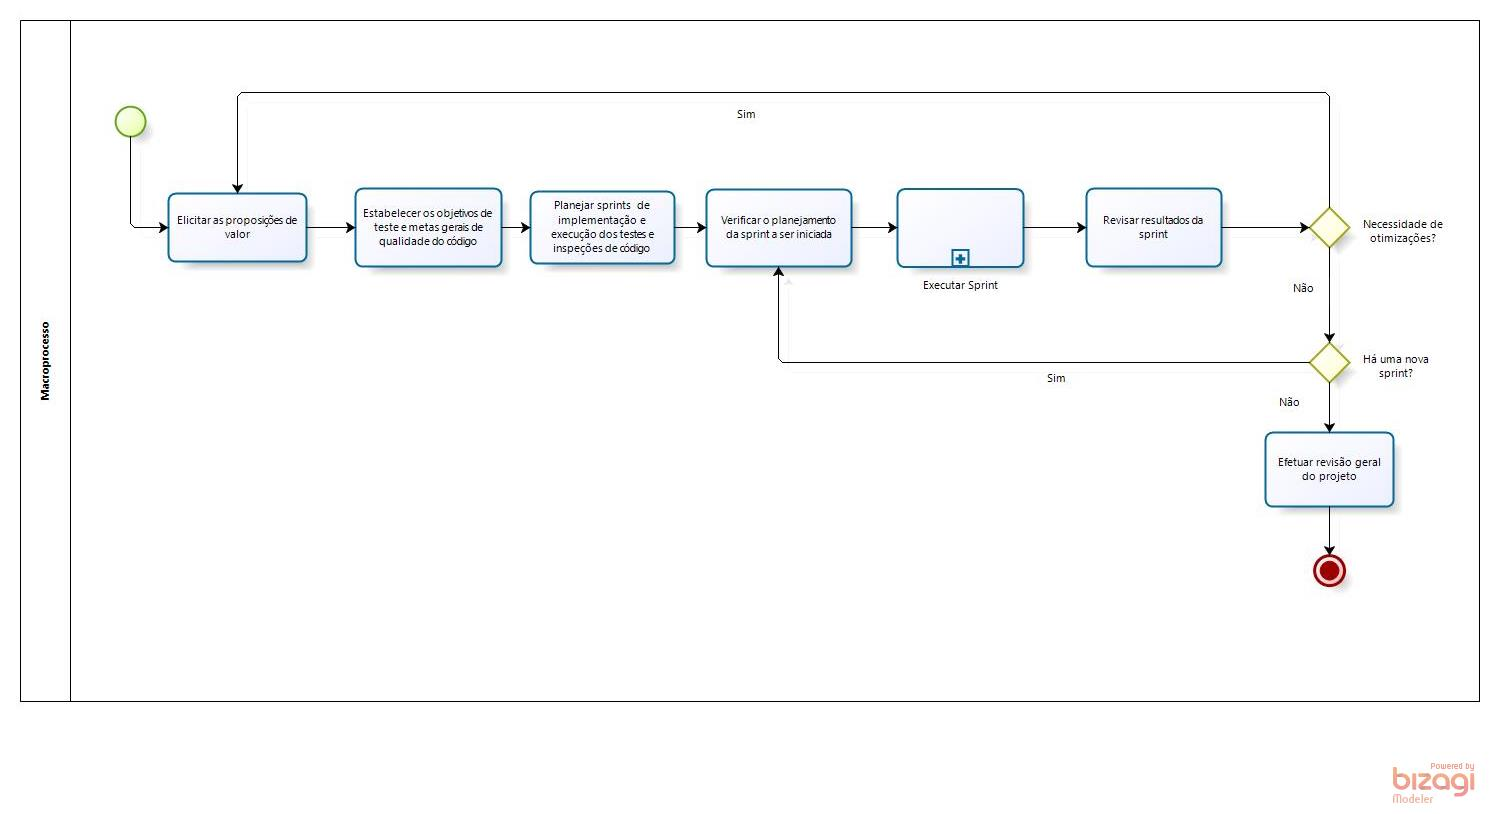
\includegraphics[width=\textwidth]{figuras/macroprocesso.jpg}
\caption{Macroprocesso - \textit{Framework de Avaliação de Código}}
\end{figure}

Iniciando a descrição das atividades pelo macroprocesso, tem-se:

\begin{itemize}
	\item \textbf{Elicitar as proposições de valor:} Caracteriza-se como uma reunião entre todos os envolvidos no projeto (área de negócio e área técnica) para alinhamento da missão do projeto. Nesta reunião, a área de negócio irá descrever quais seriam as funcionalidades mais críticas e, portanto, que mais agregam valor em seu contexto, para o \textit{software} a ser construído, de forma que a equipe técnica possa efetuar um planejamento embasado neste aspecto.

	\item \textbf{Estabelecer os objetivos de teste e metas gerais de qualidade de código:} Nesta atividade, a equipe técnica irá conceber uma estratégia para testar e assegurar a qualidade do código do \textit{software} levando em consideração os módulos priorizados a partir da elicitação das proposições de valor.

	\item \textbf{Planejar sprints de implementação e execução dos testes e inspeções de código:} Nesta atividade, o gestor do projeto, juntamente com os representantes dos demais grupos técnicos existentes no processo de desenvolvimento irão planejar as sprints, definindo início e término das mesmas, bem como os módulos do código que serão testados e inspecionados de acordo com uma priorização obtida a partir das proposições de valor.

	\item \textbf{Verificar o planejamento da sprint a ser iniciada:} Nesta atividade, o gestor do projeto irá verificar as funcionalidades a serem desenvolvidas e o que deverá ser plenamente testado e inspecionado. Assim, fará a alocação apropriada dos recursos (humanos e financeiros) para atendimento dos objetivos da sprint.

	\item \textbf{Executar Sprint:} Subprocesso que compreende as atividades corriqueiras de uma sprint segundo o Scrum, contudo, acrescentando as atividades agregadas pelo \textit{framework}.

	\item \textbf{Revisar resultados da sprint:} Nesta atividade, a equipe técnica irá verificar se todos os objetivos estabelecidos para a sprint foram alcançados, ou seja, se de fato o que foi planejado foi executado. Caso seja necessário efetuar otimizações nos planejamentos, devido também à mudança de alguma proposição de valor, a primeira atividade deverá ser executada novamente. É válido ressaltar que a interação com o cliente deve ser intensa para promover a agregação de valor em um grau satisfatório. Adicionalmente, caso algum item fique pendente, este entrará imediatamente como algo a ser concluído na sprint subsequente.

	\item \textbf{Efetuar revisão geral do projeto:} Nesta atividade, haverá uma reunião entre as áreas de negócio e técnica e todas as proposições de valor serão apresentadas de forma breve, explicitando o planejamento e a execução. Caso alguma proposição fique pendente, será avaliada a possibilidade de prorrogação de prazo para término do projeto.
\end{itemize}

A partir da descrição das atividades, é possível perceber o quão importante é fazer um bom planejamento e priorização. Caso haja mudanças no escopo e também nos prazos, a princípio, as funcionalidades que mais agregam valor já terão sido cobertas pelos instrumentos de garantia de qualidade.

Quanto à descrição das atividades constituintes do subprocesso Executar Sprint, tem-se:

\begin{itemize}
	\item \textbf{Implementar testes unitários para os módulos priorizados:} Esta atividade possui como entrada um \textit{checklist} de testes unitários, construído a partir da constatação de práticas utilizadas na indústria de desenvolvimento e que tem sido eficiente neste sentido. Assim, para a implementação dos testes unitários, espera-se o completo atendimento dos itens constantes neste \textit{checklist}.

	\item \textbf{Executar testes e coletar estatísticas:} Nesta atividade, a suíte de testes unitários será executada e aspectos pertinentes à execução desta será coletada, de forma a verificar performance, número de defeitos detectados etc.

	\item \textbf{Efetuar inspeção de código:} Nesta atividade, deverá ser feita uma inspeção do código tanto dos módulos sob teste, como também do código dos próprios métodos de teste unitário, de forma a verificar a completude e atendimento aos itens constantes no \textit{checklist} de inspeção de código.

	\item \textbf{Documentar resultados:} Além da anotação das estatísticas coletadas durante a execução dos testes, será documentado o resultado da inspeção, explicitando para cada módulo avaliado o grau de qualidade. Em caso de detecção de erros e defeitos severos, o módulo não será aprovado, ou seja, considerado finalizado e assim, deverá ser feito o aperfeiçoamento do mesmo na sprint subsequente.
\end{itemize}

A seguir, tem-se uma figura do subprocesso Executar Sprint (centralizando a atenção apenas nas atividades agregadas pelo \textit{framework}).

\begin{figure}[h]
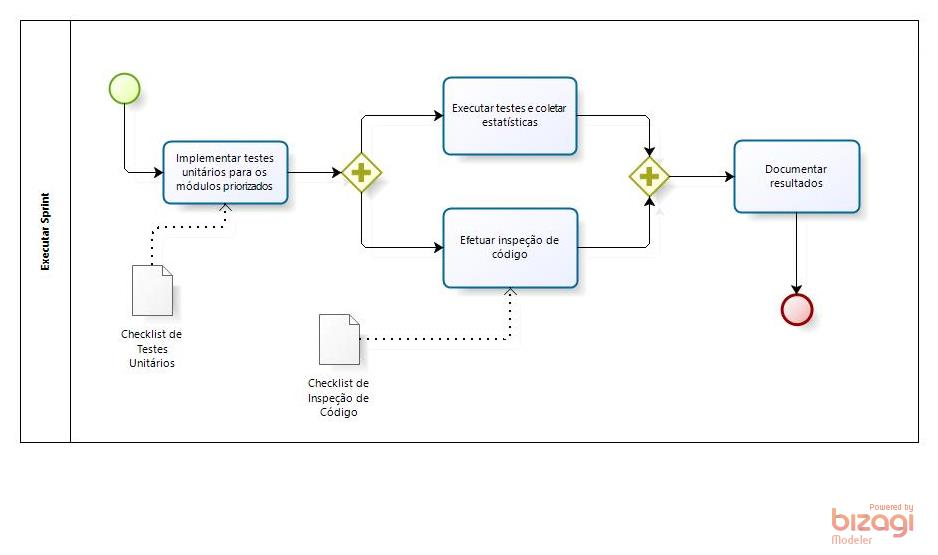
\includegraphics[width=\textwidth]{figuras/executarsprint.jpg}
\caption{Subprocesso - \textit{Executar Sprint}}
\end{figure}

\section{Coleta de Dados}